Se realizó un programa que calcula el área y perímetro de dos figuras geométricas: el trapecio y triángulo. Para ello se reciben datos del usuario mediante la herramienta \emph{Textbox} y se muestran los resultados mediante la herramienta \emph{Label}.

\textbf{Trapecio:} para calcular el área se utilizó la fórmula del área del trapecio. Para el perímetro se calculó la longitud del lado diagonal mediante el teorema de pitágoras y se sumó con los otros 2 lados y la base.

\textbf{Área del trapecio:}

\begin{equation*}
  Área = \frac{Altura 1 + Altura 2}{2} * Base
\end{equation*}

\textbf{Perímetro del trapecio:}

\begin{equation*}
  Perímetro = Lado1 + Lado2 + Base + Lado3
\end{equation*}

\textbf{Triángulo:} para calcular el área se emplea la fórmula de área del triángulo. Para el perímetro se suman los dos lados y la base.

\textbf{Área del triángulo:}

\begin{equation*}
  Área = \frac{Base * Altura}{2}
\end{equation*}

\textbf{Perímetro del triángulo:}

\begin{equation*}
  Perímetro = Lado1 + Lado2 + Base
\end{equation*}

\newpage
\textbf{Código del programa:}

\begin{lstlisting}[style=vbstyle]

  Public Class Form1
  Private Sub BtnSolucionar_Click(sender As Object, e As EventArgs) Handles BtnSolucionarTrapecio.Click
      Dim dblAlturaMayor, dblAlturaMenor As Double
      dblAlturaMayor = Convert.ToDouble(txtAlturaMayor.Text)
      dblAlturaMenor = Convert.ToDouble(txtAlturaMenor.Text)
      If dblAlturaMayor <= dblAlturaMenor Then
          If lblErrorMayorMenor.Text <> "" Then
          Else
              lblErrorMayorMenor.Text = "*Las alturas no corresponden"
          End If
      Else
          If lblErrorMayorMenor.Text <> "" Then
              lblErrorMayorMenor.Text = ""
          End If
          Dim dblArea, dblBase, dblCateto, dblHipotenusa, dblPerimetro As Double
          dblAlturaMayor = Convert.ToDouble(txtAlturaMayor.Text)
          dblAlturaMenor = Convert.ToDouble(txtAlturaMenor.Text)
          dblBase = Convert.ToDouble(txtBase.Text)
          dblCateto = dblAlturaMayor - dblAlturaMenor
          dblHipotenusa = Math.Sqrt(Math.Pow(dblBase, 2) + Math.Pow(dblCateto, 2))
          dblPerimetro = Math.Round(dblAlturaMayor + dblAlturaMenor + dblBase + dblHipotenusa, 2)
          dblArea = Math.Round(((dblAlturaMayor + dblAlturaMenor) / 2) * dblBase, 2)
          txtArea.Text = dblArea.ToString()
          txtPerimetro.Text = dblPerimetro.ToString()
          lblCatetoTrapecio.Text = Convert.ToString(Math.Round(dblCateto, 2))
          lblAlturaMayorTrapecio.Text = Convert.ToString(Math.Round(dblAlturaMayor, 2))
          lblAlturaMenorTrapecio.Text = Convert.ToString(Math.Round(dblAlturaMenor, 2))
          lblBaseTrapecio.Text = Convert.ToString(Math.Round(dblBase, 2))
          lblCatetoTrapecio.Text = Convert.ToString(Math.Round(dblCateto, 2))
          lblHipotenusaTrapecio.Text = Convert.ToString(Math.Round(dblHipotenusa, 2))
      End If
  End Sub
  Private Sub Button1_Click(sender As Object, e As EventArgs) Handles btnSolucionarTriamgulo.Click
      Dim b, h, l1, l2, area, perimetro As Double
      b = txtBaseTriangulo.Text
      h = txtAlturaTriangulo.Text
      area = (b * h) / 2
      l1 = txtLado1Triangulo.Text
      l2 = txtLado2Triangulo.Text
      perimetro = l1 + l2 + b
      txtAreaTriangulo.Text = area
      txtPerimetroTriangulo.Text = perimetro
  End Sub
End Class
  
\end{lstlisting}


\textbf{Captura de ejecución:}

\begin{figure}[H]
  \centering
  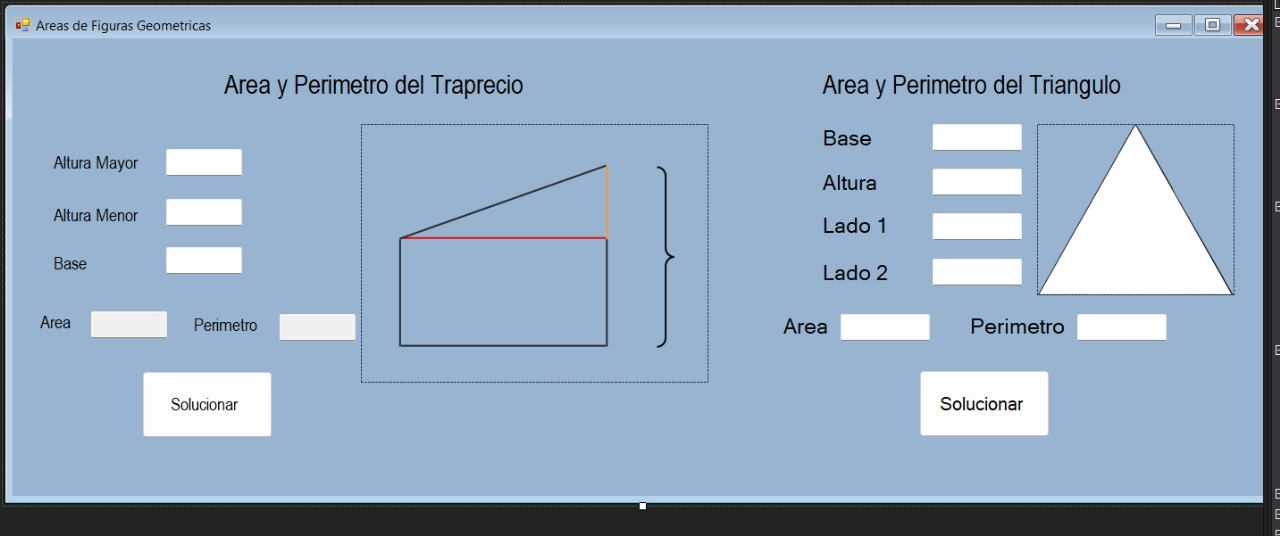
\includegraphics[scale = 0.5]{Imagenes/interfaz_grafica.jpeg}
  \caption{Interfaz Gráfica}{Fuente: Propia}
\end{figure}

\begin{figure}[H]
  \centering
  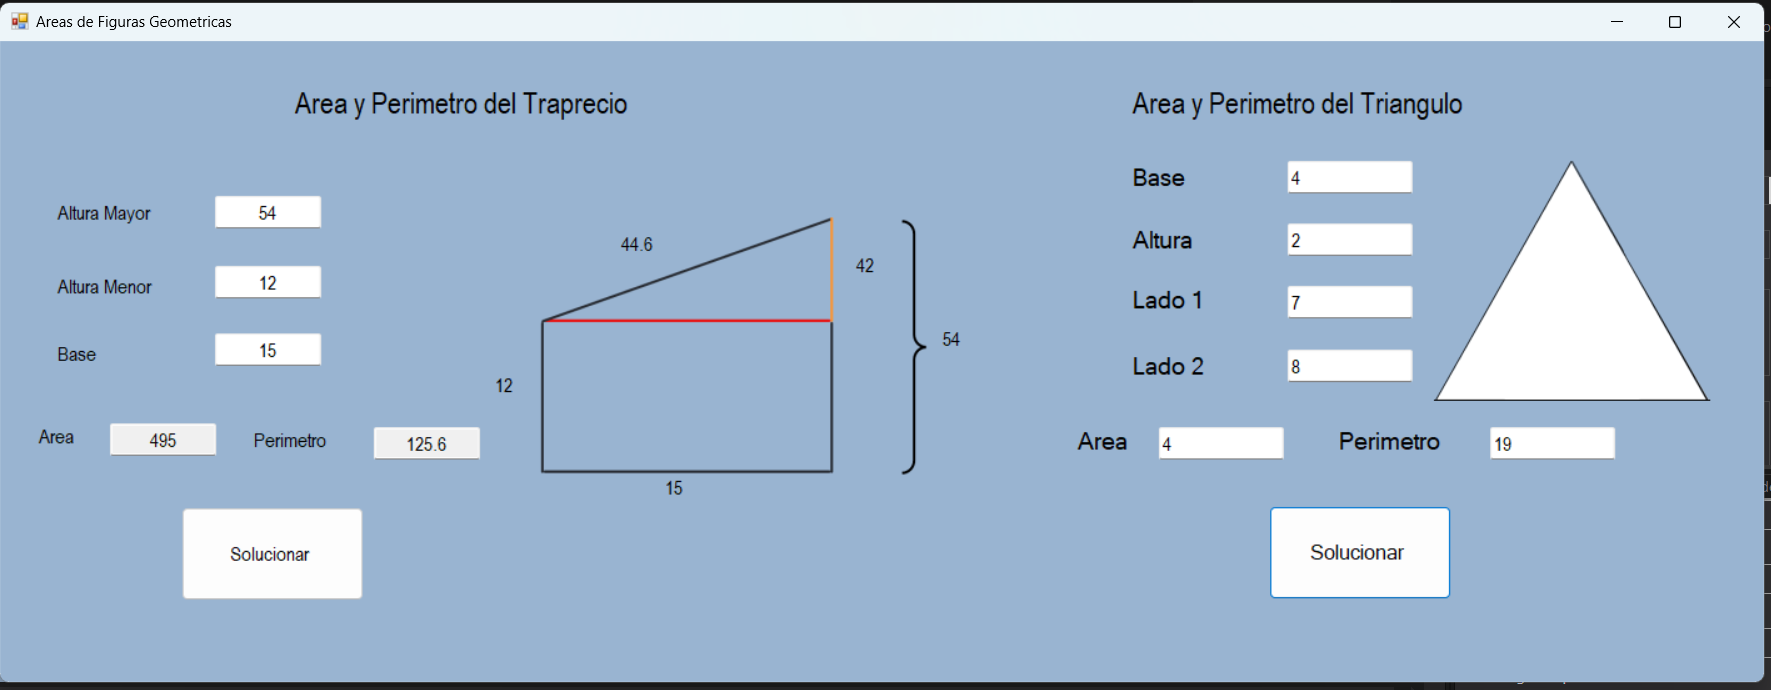
\includegraphics[scale = 0.5]{Imagenes/i2.png}
  \caption{Interfaz Gráfica}{Fuente: Propia}
\end{figure}


\begin{figure}[H]
  \centering
  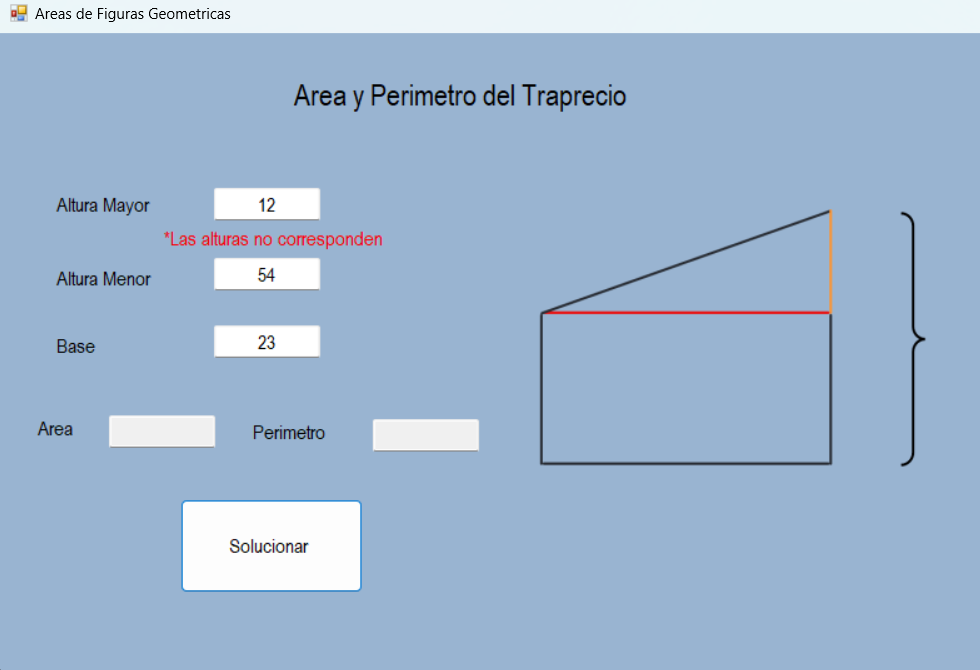
\includegraphics[scale = 0.75]{Imagenes/i3.png}
  \caption{Control de error}{Fuente: Propia}
\end{figure}